\documentclass{beamer}


% Beamer settings
\usecolortheme{rose}
\beamertemplatenavigationsymbolsempty
\setbeamertemplate{footline}[frame number]

\titlegraphic{%

\includegraphics[height=1cm]{logo-full-colour.png}}

\addtobeamertemplate{frametitle}{}{%
\begin{tikzpicture}[remember picture,overlay]
\node[anchor=north east,yshift=2pt] at (current page.north east) {
\includegraphics[height=1cm]{logo-full-colour.png}};
\end{tikzpicture}}

% Packages
\usepackage{amsmath}

\usepackage{tikz}
\usetikzlibrary{positioning}
\usetikzlibrary{fit}

\usepackage{pgfplots}
\usepgfplotslibrary{fillbetween}

\usepackage{minted}
\usepackage[T1]{fontenc} % Required by minted to ensure dollar signs are produced instead of pound (sterling) signs

\usepackage{multicol}

\usepackage{booktabs}

\usepackage{adjustbox}

% Author
\author{Simon McIntosh-Smith \& Tom Deakin\\University of Bristol}

\date{}



\title{OpenMP for Computational Scientists}
\subtitle{3: Vectorisation and optimisations}

\begin{document}

\frame{\titlepage}

%-------------------------------------------------------------------------------
\section{Outline}
\begin{frame}
\frametitle{Outline}
Now you know how to parallelise programs using OpenMP, how do you write fast programs in OpenMP?

\begin{itemize}
  \item The cache hierarchy
  \item Performance analysis
  \item Vectorisation
  \item Array of structures vs Structure of arrays
  \item Memory access patterns
  \item Memory alignment
\end{itemize}
\end{frame}

%-------------------------------------------------------------------------------
\section{Recap}
\begin{frame}
\frametitle{Recap}

\begin{itemize}
  \item Data sharing clauses:
    \begin{itemize}
    \item \mintinline{fortran}|shared|, \mintinline{fortran}|private|, \mintinline{fortran}|firstprivate|, \mintinline{fortran}|lastprivate|
    \end{itemize}

  \item Atomics and \mintinline{fortran}|critical| regions

  \item False sharing and cache thrashing

  \item Reductions with the \mintinline{fortran}|reduction| clause
\end{itemize}

Combined with the \mintinline{fortran}|parallel| and worksharing constructs from before, we've covered the OpenMP ``common core''.

\end{frame}


%-------------------------------------------------------------------------------
\begin{frame}[fragile]
\frametitle{Previous exercise}

Take your parallel 5-point stencil, and implement a reduction:
\begin{minted}[frame=single,breaklines,fontsize=\small]{fortran}
total = 0.0
!$omp parallel do collapse(2) reduction(+:total)
do i = 1, nx
  do j = 1, ny
    Atmp(i,j) = (A(i-1,j) + A(i+1,j) + A(i,j) + A(i,j-1) + A(i,j+1)) / 5.0
    total = total + Atmp(i,j)
  end do
end do
!$omp end parallel do
\end{minted}

\begin{itemize}
  \item Well done if you managed this!
  \item 5-point stencil is simple, but captures the \emph{essence} of more complicated codes.
  \item Extension: did anyone try the parallelising the Jacobi solver?
\end{itemize}

\end{frame}

%-------------------------------------------------------------------------------
\section{The cache hierarchy}
\begin{frame}
\frametitle{Cache hierarchy}
\begin{center}
\begin{adjustbox}{max width={.8\textwidth}}
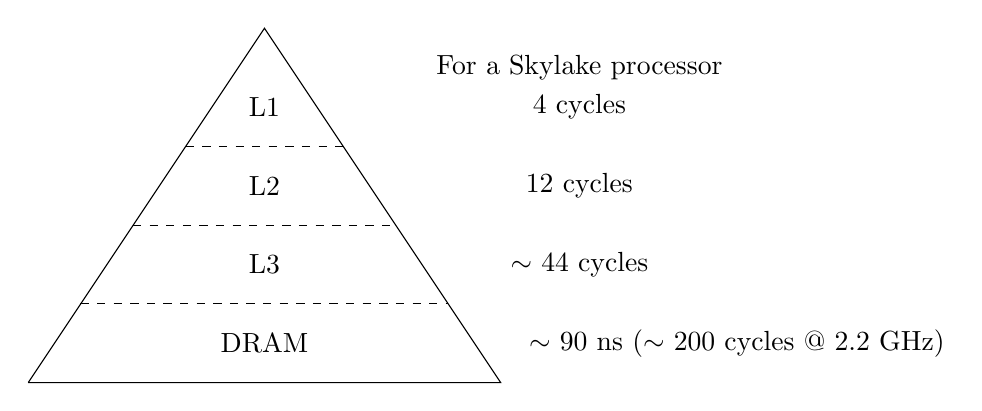
\begin{tikzpicture}
  % Triangle
  \draw (-3,0) -- (0,4.5) -- (3,0) -- (-3,0);

  \node at (4,4) {For a Skylake processor};
  \node at (0,3.5) {L1};
  \node at (4,3.5) {4~cycles};

  \draw[dashed] (-1,3) -- (1,3);
  \node at (0,2.5) {L2};
  \node at (4,2.5) {12~cycles};

  \draw[dashed] (-1.67,2) -- (1.67,2);
  \node at (0,1.5) {L3};
  \node at (4,1.5) {$\sim$ 44~cycles};

  \draw[dashed] (-2.337,1) -- (2.337,1);
  \node at (0,0.5) {DRAM};
  \node at (6,0.5) {$\sim$ 90~ns ($\sim$ 200 cycles @ 2.2~GHz)};
\end{tikzpicture}
\end{adjustbox}
\end{center}

\begin{itemize}
  \item Most integer and floating point operations are single cycle.
  \item Memory access is relatively slow.
  \item Moving memory between nodes is hugely expensive: $\sim 3\mu s$
  \item How long is a nanosecond? 11.8 inches --- Grace Hopper: \url{https://youtu.be/JEpsKnWZrJ8}.
  \item Therefore very easy to become bound by memory movement.

\end{itemize}
\end{frame}

%-------------------------------------------------------------------------------
\begin{frame}
\frametitle{Cache bandwidth}

Graph of aggregate cache bandwidth on different architectures:
\begin{center}
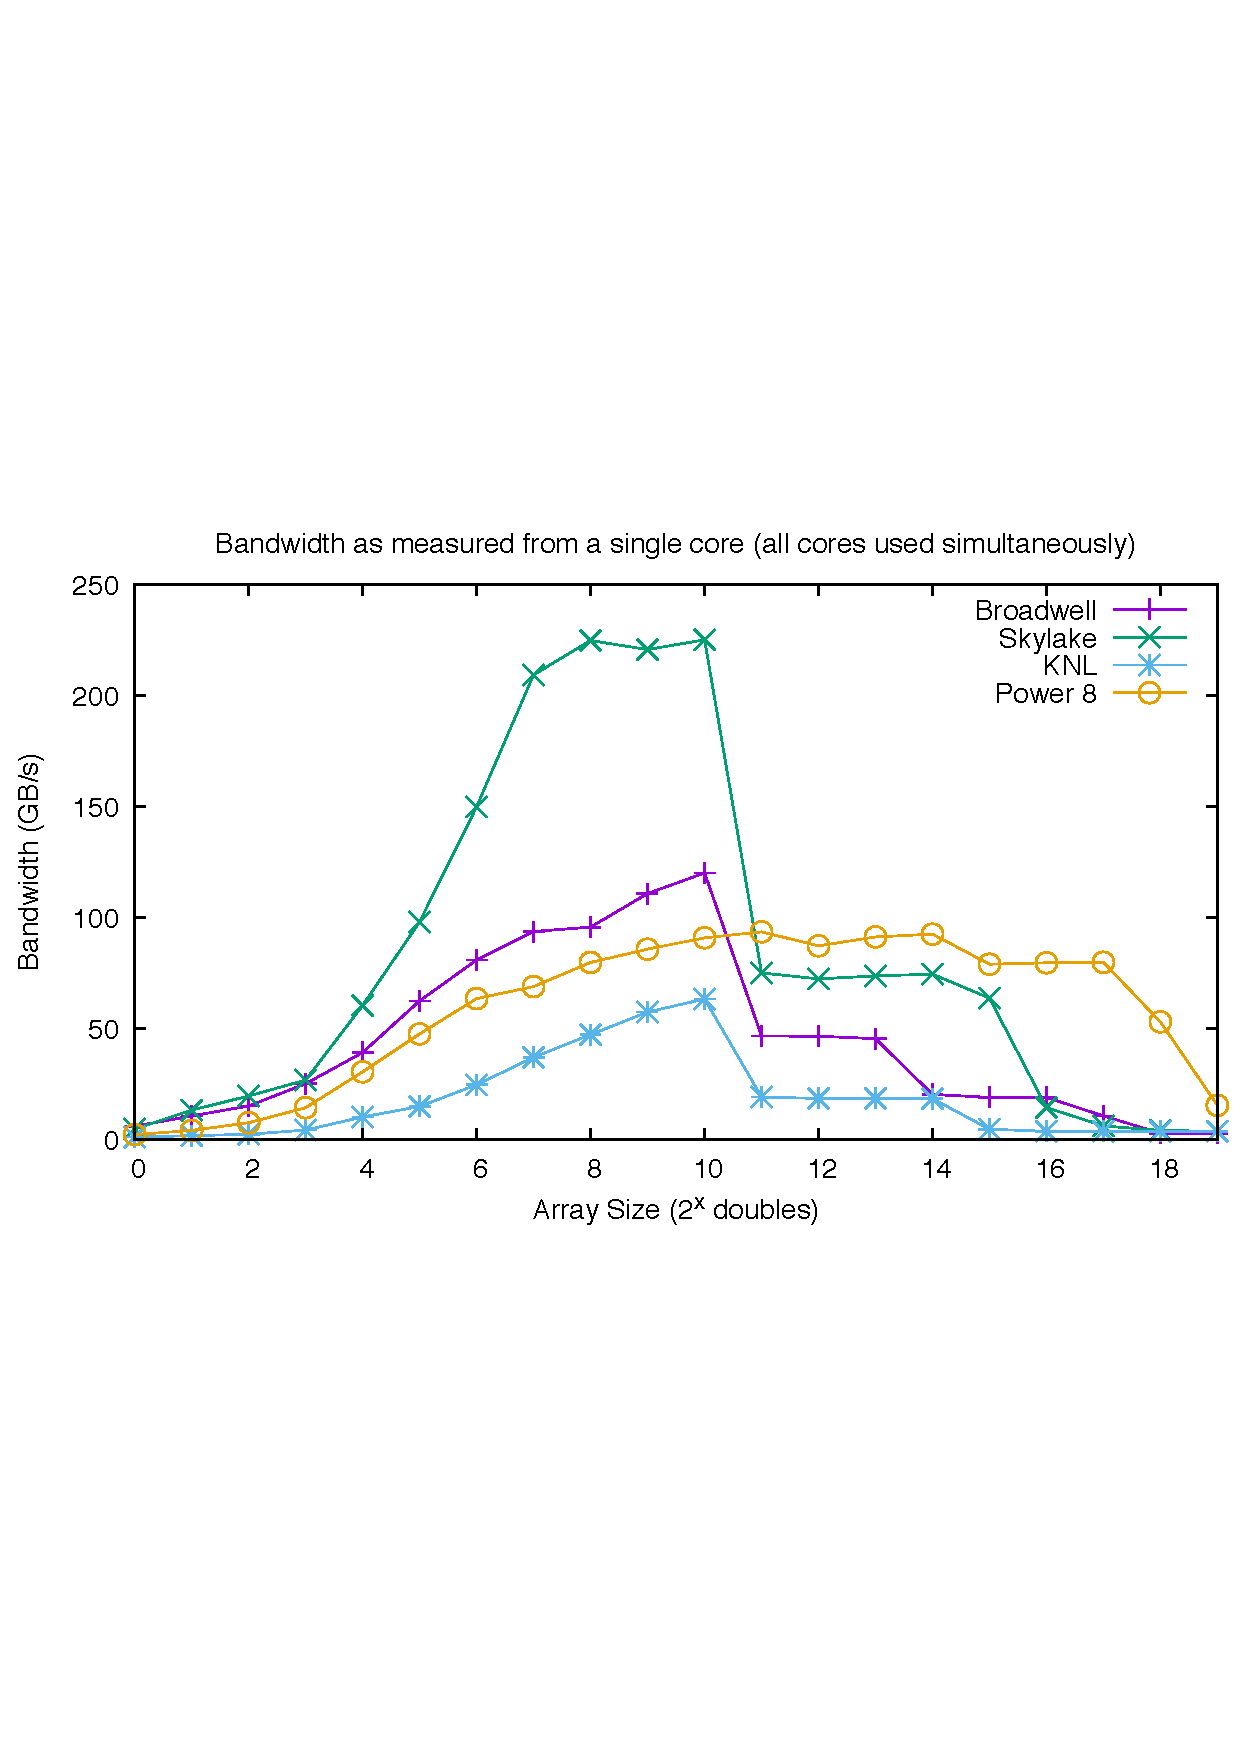
\includegraphics[width=0.8\textwidth]{cache_bandwidth}
\end{center}

\begin{itemize}
  \item Clear cliff edges at cache capacity sizes (3 times x-axis).
  \item As with latency: more performance from lower levels.
\end{itemize}


\footnotetext[1]{{\Tiny Deakin, T., Price, J., and McIntosh-Smith, S. (2017). Portable Methods for Measuring Cache Hierarchy Performance (poster).\\In Supercomputing. Denver, CO.}}

\end{frame}

%-------------------------------------------------------------------------------
\begin{frame}[fragile]
\frametitle{Streaming data}

STREAM Triad kernel:

\begin{minted}[frame=single]{fortran}
!$omp parallel do
do i = 1, N
  a(i) = b(i) + scalar * c(i)
end do
!$omp end parallel do
\end{minted}

\begin{itemize}
  \item Where \mintinline{fortran}|N| is large, the arrays exceed cache capacity.
  \item This kernel has \emph{no} data reuse: data items are read or written once, then never used again.
  \item Example of a \emph{streaming} data access pattern.
  \item Performance is then bound by main memory bandwidth.
\end{itemize}

\end{frame}

%-------------------------------------------------------------------------------
\section{Performance analysis}
\begin{frame}
\frametitle{Performance analysis}
\begin{itemize}
  \item Optimisations can help code go faster, but how do you know when it's performing \emph{well}?
  \item Helpful to think about characteristics of the algorithm:
    \begin{itemize}
      \item Algorithmic complexity for compute.
      \item Algorithmic complexity for data movement.
    \end{itemize}
  \item Examples:
    \begin{itemize}
      \item Vector-vector and vector-matrix are $O(n)$ for compute and data movement.
      \item Matrix-matrix multiply is $O(n^3)$ for compute and $O(n^2)$ for data movement.
      \item Matrix multiplication becomes \emph{compute bound} at large enough $n$, but other examples remain memory bandwidth bound.
    \end{itemize}
\end{itemize}
\end{frame}

%-------------------------------------------------------------------------------
\begin{frame}
\frametitle{Rate limiting factors}
\begin{itemize}
  \item Most HPC codes are \emph{memory bandwidth bound}.
  \item A few are \emph{compute bound}.
  \item Other possibilities:
    \begin{itemize}
      \item Network bound (e.g. MPI communication).
      \item I/O bound (e.g. writing to the filesystem).
      \item Memory latency bound.
      \item Memory capacity bound.
      \item \dots
    \end{itemize}
  \item Worth thinking about the bound for your own code.
  \item Arithmetic (integer and floating point) is very cheap $O(1)$ cycle.
  \item Division, transcendentals, exponentials/logs are relatively slow.
  \item Load/store is 2--3 times slower than an arithmetic operation, even if it's an L1 cache hit (the best case).
  \item Consider the ratio of bytes moved vs. floating point operations.
\end{itemize}
\end{frame}
%-------------------------------------------------------------------------------
\begin{frame}
\frametitle{Computational intensity}
\begin{itemize}
  \item The radio of FLOPS to bytes moved is known as \emph{computational intensity}, or CI.
  \item Originally only DRAM traffic counted, but this causes problems.
  \item Bytes moved is best calculated from the kernel perspective.
  \item Take this example:
    \begin{itemize}
      \item \mintinline{fortran}|a(i) = a(i) + b(i) * c(i)|
      \item Assume FP64 arrays.
      \item Count the data movement and floating point operations for each \mintinline{fortran}|i|.
      \item 24 bytes loaded, 8 bytes stored.
      \item Two floating point operations: one \mintinline{fortran}|+| and one \mintinline{fortran}|*|.
      \item CI of $2/32 = 1/16$.
    \end{itemize}
\end{itemize}
\end{frame}

%-------------------------------------------------------------------------------
\begin{frame}
\frametitle{Roofline model}
Useful conceptual tool to establish whether compute or memory bandwidth bound.

\begin{center}
\begin{adjustbox}{max width={.6\textwidth}}
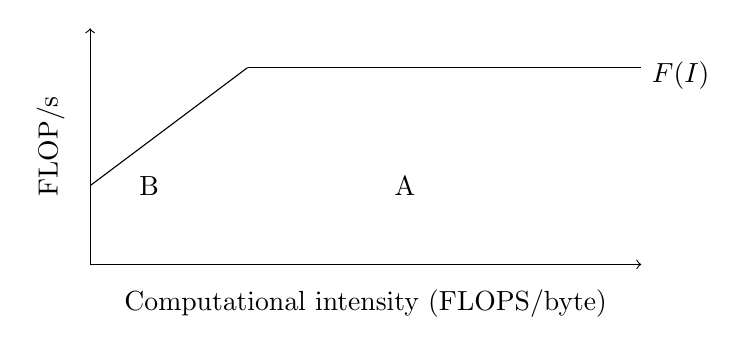
\begin{tikzpicture}
  \draw[->] (0,0)   -- (0,3);
  \draw[->] (0,0)   -- (7,0);
  \draw     (0,1)   -- (2,2.5);
  \draw     (2,2.5) -- (7,2.5);
  \node at (3.5,-0.5) {Computational intensity (FLOPS/byte)};
  \node[rotate=90] at (-0.5,1.5) {FLOP/s};
  \node at (7.5,2.4) {$F(I)$};
  \node at (4,1) {A};
  \node at (0.75,1) {B};
\end{tikzpicture}
\end{adjustbox}
\end{center}

\begin{itemize}
  \item The roof $F(I)$ is found from tech sheet data and/or micro-benchmarks.
  \item Runtime performance of kernel gives FLOP/s, analysis of bytes/FLOPS gives CI.
  \item Kernel A is compute bound; Kernel B is memory bandwidth bound.
  \item Both kernels require optimisation!
  \item If kernel is on the roof, then rate limiting factor is achieved.
\end{itemize}
\end{frame}

%-------------------------------------------------------------------------------
\begin{frame}
\frametitle{Intel Advisor: Roofline}
\begin{itemize}
  \item Can use Intel Advisor to run a Roofline analysis on your code.
  \item First, it runs some micro-benchmarks to generate the Roofline model.
  \item Then, it runs your code, calculating the CI and performance.
  \item Can be helpful to visualise how performant your code is.
  \item More information: \url{https://software.intel.com/en-us/articles/intel-advisor-roofline}.
  \item But beware, the CI is calculated from executed instructions, so not always the whole picture.
\end{itemize}
\end{frame}

%-------------------------------------------------------------------------------
\section{Vectorisation}
\begin{frame}
\frametitle{Vectorisation}
$$C=A+B$$
\begin{columns}
\begin{column}{0.5\textwidth}
Scalar operations \\
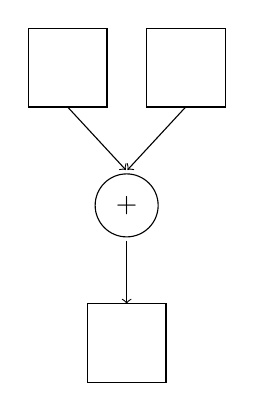
\begin{tikzpicture}
  \draw (-0.5,2) rectangle (0.5,3);
  \draw (1,2) rectangle (2,3);
  \draw[->] (0,2) -- (.74,1.2);
  \draw[->] (1.5,2) -- (.76,1.2);
  \draw (.75,.75) circle (.4cm);
  \draw (.75,.75) node {$+$};
  \draw[->] (.75,0.3) -- (.75,-0.5);
  \draw (.25,-1.5) rectangle (1.25,-0.5);
\end{tikzpicture}
\end{column}

\begin{column}{0.5\textwidth}
Vector operations \\
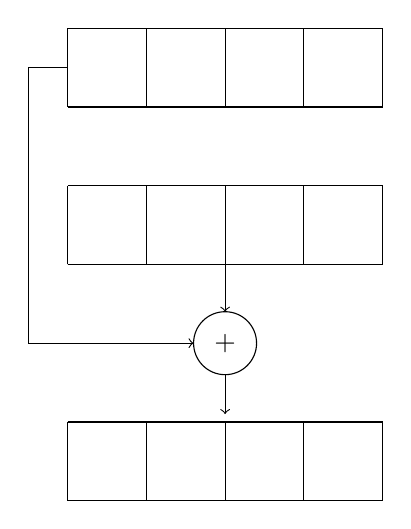
\begin{tikzpicture}
  \draw[step=1cm] (0,2) grid (4,3);
  \draw[step=1cm] (0,0) grid (4,1);
  \draw[->] (2,0) -- (2,-0.6);
  \draw[->] (0,2.5) -- (-0.5,2.5) -- (-0.5,-1) -- (1.6,-1);
  \draw (2,-1) circle (.4cm);
  \draw (2,-1) node {$+$};
  \draw[->] (2,-1.4) -- (2,-1.9);
  \draw[step=1cm] (0,-3) grid (4,-2);
\end{tikzpicture}
\end{column}
\end{columns}

\end{frame}

%-------------------------------------------------------------------------------
\begin{frame}
\frametitle{Why vectorise?}
\begin{itemize}
  \item Vectorisation gives you more compute per cycle.
  \item Hence may increase the FLOP/s rate of the processor.
  \item Also results in fewer instructions to process (less pressure on instruction decode units).
  \item Vectors help make good use of the memory hierarchy (often the main benefit).
  \item Vectorisation helps you write code which has good access patterns to maximise bandwidth.
\end{itemize}
\end{frame}

%-------------------------------------------------------------------------------
\begin{frame}
\frametitle{Auto-vectorisation}
\begin{itemize}
  \item Modern compilers are very good at automatically vectorising your loops.
  \item Fortran helps as arrays can not alias (overlap), unlike C.
  \item But compiler needs to be sure it's safe to vectorise.
  \item Read compiler reports to see if it's already vectorising.
    \begin{itemize}
      \item Intel: \mintinline{bash}|-qopt-report=5|
      \item Cray: \mintinline{bash}|-hlist=a|
      \item GNU (old): \mintinline{bash}|-ftree-vectorizer-verbose=2|
      \item GNU (new): \mintinline{bash}|-fopt-info-vec|
    \end{itemize}
  \item Often the memory access pattern prevents (efficient) auto-vectorisation.
\end{itemize}
\end{frame}

%-------------------------------------------------------------------------------
\subsection{OpenMP SIMD}
\begin{frame}[fragile]
\frametitle{OpenMP SIMD}
\begin{itemize}
  \item Sometimes the compiler needs help in confirming loops are vectorisable.
  \item OpenMP \mintinline{fortran}|simd| constructs give this information.
  \item Can combine with \mintinline{fortran}|parallel do| construct to ensure a parallel vector loop: \mintinline{fortran}|omp parallel do simd|
  \item Generally want to vectorise inner loops and parallelise outer loops.
\end{itemize}

\begin{minted}[frame=single]{fortran}
!$omp simd
do i = 1, N
  C(i) = A(i)+B(i)
end do
!$omp end simd
\end{minted}
\end{frame}

%-------------------------------------------------------------------------------
\begin{frame}[fragile]
\frametitle{SIMD functions}
Say you've written an update function to update values in the loop:
\begin{minted}[frame=single]{fortran}
do i = 1, N
  A(i) = magic_maths(A(i))
end do
\end{minted}

\begin{itemize}
  \item The situation gets complicated.
  \item If the function is small, then likely inlined and loop will auto-vectorise.
  \item Otherwise need to use the \mintinline{fortran}|simd| construct, but need compiler to create a vector version of the function.
\end{itemize}

\begin{minted}[frame=single]{fortran}
function magic_maths(value) result(r)
!$omp declare simd(magic_maths)
  implicit none
  real(kind=8) :: value, r
  r = value * value
end function
\end{minted}

\end{frame}

%-------------------------------------------------------------------------------
\begin{frame}[fragile]
\frametitle{SIMD clauses}
\begin{itemize}
  \item All the usual data-sharing and reduction clauses can be applied.
  \item \mintinline{fortran}|safelen(4)|: distance between iterations where its safe to vectorise.
  \begin{minted}[frame=single]{fortran}
  !$omp simd safelen(4)
  do i = 1, N-4
    A(i) = A(i) + A(i+4)
  end do
  !$omp end simd
  \end{minted}
  \item \mintinline{fortran}|simdlen(4)|: preferred iterations to be performed concurrently as a vector.
  Specifying explicit vector lengths builds in obsolescence to the code as hardware vector lenghts continually change --- don't recommend using this clause.
\end{itemize}
\end{frame}

%-------------------------------------------------------------------------------
\begin{frame}[fragile]
\frametitle{SIMD clauses}
\begin{itemize}
  \item \mintinline{fortran}|linear(var)|: variable is private and linear to the loop iterator.
  \begin{minted}[frame=single]{fortran}
  !$omp simd linear(j)
  do i = 1, N
    j = j + 1
    A(j) = B(i)
  end do
  !$omp end simd
  \end{minted}
  \item \mintinline{fortran}|aligned(var)|: says the array is aligned (more on this shortly).
  \item \mintinline{fortran}|uniform(var)|: for \mintinline{fortran}|declare simd| construct, the variable is the same in all vector lanes.
\end{itemize}
\end{frame}

%-------------------------------------------------------------------------------
\begin{frame}
\frametitle{SIMD summary}

\begin{itemize}
  \item Sometimes need to force the compiler to auto-vectorise (the correct) loop with the \mintinline{fortran}|simd| construct.
  \item As with \mintinline{fortran}|parallel|, you are telling the compiler it is safe to vectorise and to ignore its data dependancy analysis.
  \item Check the compiler report before and after the check it did the right thing!
  \item Use \mintinline{fortran}|declare simd| and appropritae clauses if you need to create vectorised versions of functions.
  \begin{itemize}
    \item The clauses can give more information to the compiler so it does a better job.
  \end{itemize}
\end{itemize}

\end{frame}

%-------------------------------------------------------------------------------
\section{Derived types}
\begin{frame}[fragile]
\frametitle{Derived types}
2D grid of cells, each cell containing 4 different values.
\begin{minted}[frame=single,linenos,fontsize=\small]{fortran}
type cell
  real(kind=8) :: property1
  real(kind=8) :: property2
  real(kind=8) :: property3
  real(kind=8) :: property4
end type

type(cell), allocatable :: grid(:,:)

do j = 1, ny
  do i = 1, nx
    grid(i,j)%property1 = update_1()
    grid(i,j)%property2 = update_2()
    grid(i,j)%property3 = update_3()
    grid(i,j)%property4 = update_4()
  end do
end do
\end{minted}
\end{frame}

%-------------------------------------------------------------------------------
\begin{frame}
\frametitle{Derived types}
\begin{itemize}
  \item What do Fortran derived types look like in memory?
  \item Organised as an array of structures.
  \item<2-> What happens when we vectorise our loop over cells?
\end{itemize}

\begin{adjustbox}{max width={\textwidth}}
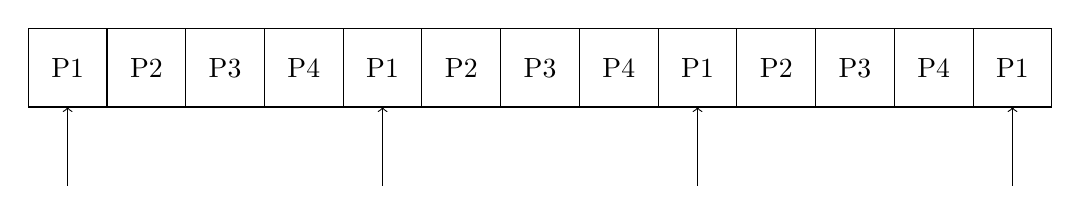
\begin{tikzpicture}
  \draw[step=1cm] (0,0) grid (13,1);
  \foreach \i in {0,4,8,12} {
    \draw (\i+.5,.5) node {P1};
  }
  \foreach \i in {0,4,8} {
    \draw (\i+1.5,.5) node {P2};
    \draw (\i+2.5,.5) node {P3};
    \draw (\i+3.5,.5) node {P4};
  }

  \foreach \i in {0,4,8,12} {
    \draw<3->[->] (\i+.5,-1) -- (\i+.5,0);
  }
\end{tikzpicture}
\end{adjustbox}

\begin{itemize}
  \item<4-> The \mintinline{fortran}|property1| values are gathered into a vector register.
  \item<5-> After the computation, the results are scattered back into memory.
  \item<6-> A cache line is 64 bytes, so only the first two values are on the first cache line.
  \item<6-> Must read two cache lines to fill the vector up.
\end{itemize}
\end{frame}

%-------------------------------------------------------------------------------
\begin{frame}[fragile]
\frametitle{Structure of arrays}
Switch type around to have an array per property.
\begin{minted}[frame=single,linenos]{fortran}
type grid
  real(kind=8), allocatable :: property1(:,:)
  real(kind=8), allocatable :: property2(:,:)
  real(kind=8), allocatable :: property3(:,:)
  real(kind=8), allocatable :: property4(:,:)
end type

do j = 1, ny
  do i = 1, nx
    grid%property1(i,j) = update_1()
    grid%property2(i,j) = update_2()
    grid%property3(i,j) = update_3()
    grid%property4(i,j) = update_4()
  end do
end do
\end{minted}
\end{frame}

%-------------------------------------------------------------------------------
\begin{frame}
\frametitle{Structure of arrays}
\begin{itemize}
  \item Order of data in memory has changed.
  \item<2-> What happens when we vectorise?
\end{itemize}

\begin{adjustbox}{max width={\textwidth}}
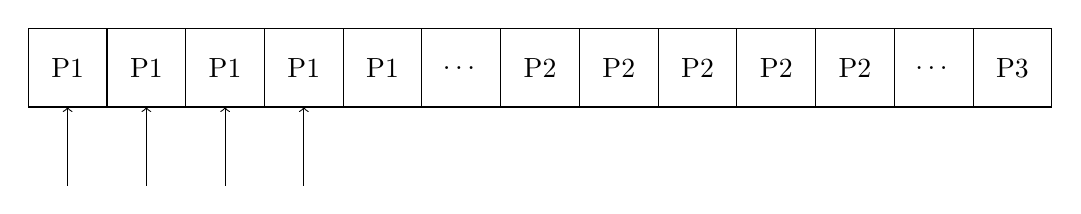
\begin{tikzpicture}
  \draw[step=1cm] (0,0) grid (13,1);
  \foreach \i in {0,...,4} {
    \draw (\i+.5,.5) node {P1};
  }
  \draw (5.5,.5) node {\dots};

  \foreach \i in {5,...,9} {
    \draw (\i+1.5,.5) node {P2};
  }
  \draw (11.5,.5) node {\dots};

  \foreach \i in {10} {
    \draw (\i+2.5,.5) node {P3};
  }

  \foreach \i in {0,...,3} {
    \draw<3->[->] (\i+.5,-1) -- (\i+.5,0);
  }
\end{tikzpicture}
\end{adjustbox}

\onslide<4->{
\begin{itemize}
  \item Coalesced memory accesses are key for high performance code.
  \item Adjacent vector lanes read adjacent memory locations.
  \item A cache line is 64 bytes, so can fill the vector from a single cache line.
  \item More efficient vectorisation.
\end{itemize}
}
\end{frame}

%-------------------------------------------------------------------------------
\section{Memory access patterns}
\begin{frame}[fragile]
\frametitle{Memory access patterns}
\begin{minted}{fortran}
do i = 1, N
  val = A(i)
end do
\end{minted}
\begin{adjustbox}{max width={\textwidth}}
\begin{tikzpicture}
  \draw[step=1cm] (-3,0) grid (11,1);
  \draw[dashed] (0,-.5) -- (0,1.5);
  \draw[dashed] (8,-.5) -- (8,1.5);
  \draw (0,-1) node {64 byte boundary};
  \foreach \i in {0,...,7} {
    \draw[->] (\i+.5,2) -- (\i+.5,1.2);
  }
\end{tikzpicture}
\end{adjustbox}
\begin{itemize}
  \item Ideal memory access pattern.
  \item All access is coalesced.
  \item Vectors are aligned to cache line boundary.
\end{itemize}
\end{frame}

%-------------------------------------------------------------------------------
\begin{frame}[fragile]
\frametitle{Memory access patterns}
\begin{minted}{fortran}
do i = 1, N
  val = A(i+3)
end do
\end{minted}
\begin{adjustbox}{max width={\textwidth}}
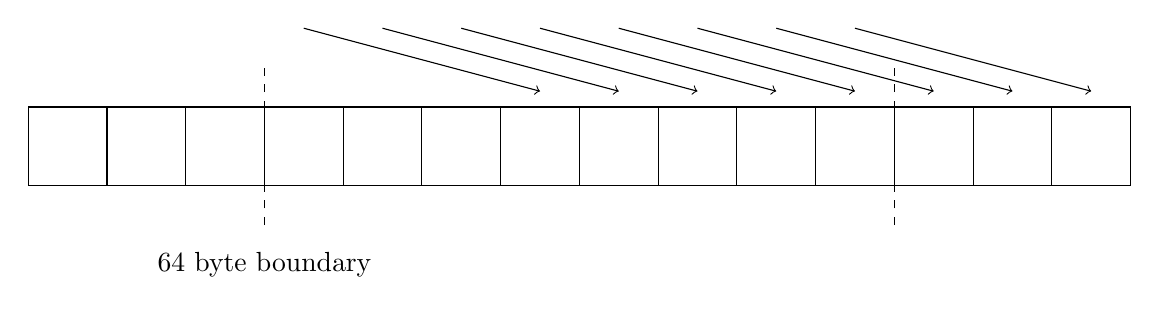
\begin{tikzpicture}
  \draw[step=1cm] (-3,0) grid (11,1);
  \draw[dashed] (0,-.5) -- (0,1.5);
  \draw[dashed] (8,-.5) -- (8,1.5);
  \draw (0,-1) node {64 byte boundary};
  \foreach \i in {0,...,7} {
    \draw[->] (\i+.5,2) -- (3+\i+.5,1.2);
  }
\end{tikzpicture}
\end{adjustbox}
\begin{itemize}
  \item OK memory access pattern.
  \item All access is coalesced, but split across cache lines.
  \item Still get good use of cache lines, but not as efficient as aligned version.
\end{itemize}
\end{frame}

%-------------------------------------------------------------------------------
\begin{frame}[fragile]
\frametitle{Memory access patterns}
\begin{minted}{fortran}
do i = 1, N
  val = A(j,i) ! equiv. A(j+3*i)
end do
\end{minted}
\begin{adjustbox}{max width={\textwidth}}
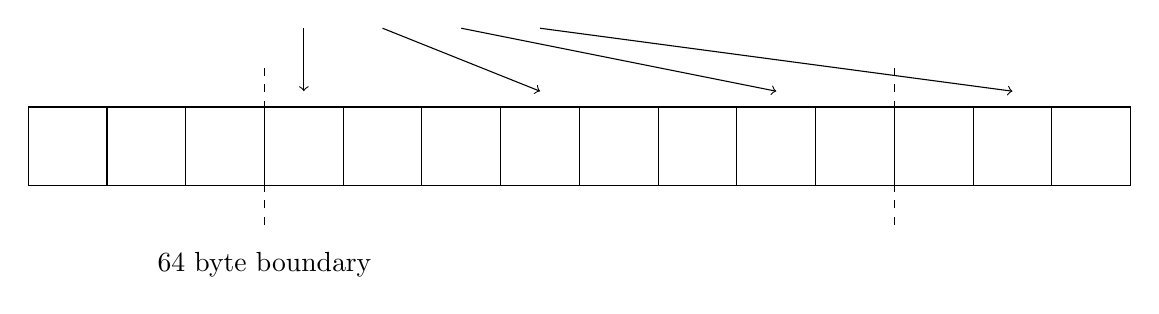
\begin{tikzpicture}
  \draw[step=1cm] (-3,0) grid (11,1);
  \draw[dashed] (0,-.5) -- (0,1.5);
  \draw[dashed] (8,-.5) -- (8,1.5);
  \draw (0,-1) node {64 byte boundary};
  \foreach \i in {0,...,3} {
    \draw[->] (\i+.5,2) -- (3*\i+.5,1.2);
  }
\end{tikzpicture}
\end{adjustbox}
\begin{itemize}
  \item Strided access results in multiple memory transactions.
  \item Kills throughput due to poor reuse of cached data.
  \item Very easy to fall into this trap with multi-dimensional arrays.
  \item Check your strides!
\end{itemize}
\end{frame}

%-------------------------------------------------------------------------------
\begin{frame}[fragile]
\frametitle{Memory access patterns}
\begin{minted}{fortran}
do i = 1, N
  val = A(B(i))
end do
\end{minted}
\begin{adjustbox}{max width={\textwidth}}
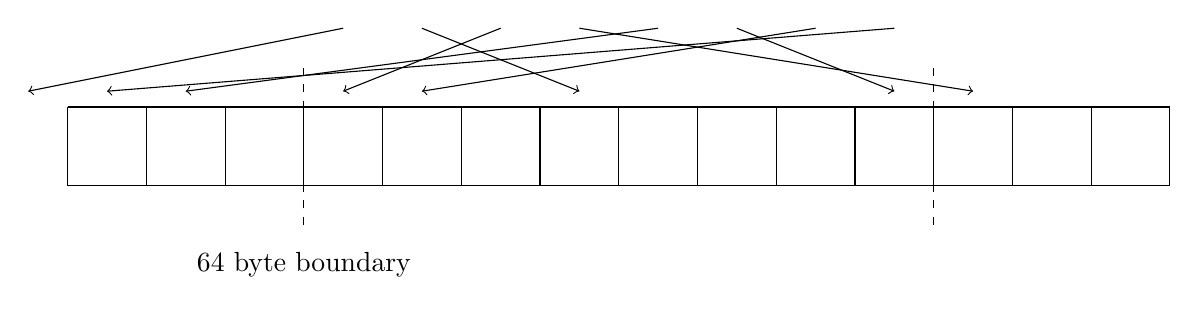
\begin{tikzpicture}
  \draw[step=1cm] (-3,0) grid (11,1);
  \draw[dashed] (0,-.5) -- (0,1.5);
  \draw[dashed] (8,-.5) -- (8,1.5);
  \draw (0,-1) node {64 byte boundary};
  \draw[->] (0.5,2) -- (-3.5,1.2);
  \draw[->] (1.5,2) -- (3.5,1.2);
  \draw[->] (2.5,2) -- (0.5,1.2);
  \draw[->] (3.5,2) -- (8.5,1.2);
  \draw[->] (4.5,2) -- (-1.5,1.2);
  \draw[->] (5.5,2) -- (7.5,1.2);
  \draw[->] (6.5,2) -- (1.5,1.2);
  \draw[->] (7.5,2) -- (-2.5,1.2);
\end{tikzpicture}
\end{adjustbox}
\begin{itemize}
  \item Essentially random access to memory.
  \item Little reuse of cache lines.
  \item Unpredictable pattern, so hardware prefetchers won't work efficiently.
  \item Very challenging!
\end{itemize}
\end{frame}

%-------------------------------------------------------------------------------
\section{Alignment}
\begin{frame}
\frametitle{Alignment}
\begin{itemize}
  \item If we can align arrays, we get better vectorisation; specifically load/stores are faster.
    \begin{itemize}
      \item Guarantee only one cache line needs updating and not split between two cache lines.
    \end{itemize}
  \item Taking advantage of alignment is a two stage process:
    \begin{enumerate}
      \item Align the memory on allocation.
      \item Tell the compiler the access is aligned.
    \end{enumerate}
  \item Aligned allocations in Fortran are (currently) unfortunately vendor specific.
  \item OpenMP can help with telling the compiler the data is aligned.
  \item Aligned allocations due in OpenMP 5.0.
\end{itemize}
\end{frame}

%-------------------------------------------------------------------------------
\begin{frame}[fragile]
\frametitle{Step 1: Aligning allocations}
Generally focus on the Intel compiler.
Only need to use one of these methods, whichever is most convenient.
\begin{itemize}
  \item Align all allocations of arrays (not in derived types) with compiler flag: \mintinline{bash}|-align array64byte|
  \item Use an Intel compiler directive on array definition:
  \begin{minted}[frame=single,fontsize=\small]{fortran}
  real(kind=8), allocatable :: A(:,:)
  !dir$ attributes align:64 :: A
  \end{minted}
  \item Allocate memory in C, and convert to Fortran \mintinline{fortran}|pointer|:
  \begin{minted}[frame=single,breaklines,fontsize=\small]{c}
  double * alloc(int *len) {
    return (double *)aligned_alloc(64, sizeof(double)*(*len));
  }
  \end{minted}
  \begin{minted}[frame=single,fontsize=\small]{fortran}
  real(kind=8), pointer :: A(:,:)
  type(c_ptr) :: A_ptr
  A_ptr = alloc(nx*ny)
  call c_f_pointer(A_ptr, A, (/ nx, ny/))
  \end{minted}
\end{itemize}
\end{frame}

%-------------------------------------------------------------------------------
\begin{frame}[fragile]
\frametitle{Step 2: Telling the compiler}
\begin{itemize}
  \item Use OpenMP \mintinline{fortran}|simd aligned| clause:
  \begin{minted}[frame=single,fontsize=\small]{fortran}
  !$omp simd aligned(A:64)
  do i = 1, nx
    A(i,j) = A(i,j) + 1.0
  end do
  !$omp end simd
  \end{minted}
  \pause
  \item Unfortunately often not sufficient.
  \item Often need to use Intel specific directives to say loop extent is divisible by vector length.
  \begin{minted}[frame=single,fontsize=\small]{fortran}
  ! 64 byte aligned / 8 byte data type means mod 8
  !dir$ assume(mod(nx,8) .eq. 0)
  !$omp simd aligned(A:64)
  do i = 1, nx
    A(i,j) = A(i,j) + 1.0
  end do
  !$omp end simd
  \end{minted}
  \item Check the compiler report for aligned and unaligned access.
\end{itemize}
\end{frame}

%-------------------------------------------------------------------------------
\begin{frame}[fragile]
\frametitle{Aligning 2D arrays}
\begin{itemize}
  \item Aligning the memory only aligns the first entry.
  \item Multiples of the alignment factor will also be aligned.
  \item With 2D arrays you need to double check that access can be aligned.
  \item Example: 10-by-10 grid of FP64 numbers, aligned to 64 byte cache line:
\end{itemize}

\begin{adjustbox}{max width={\textwidth}}
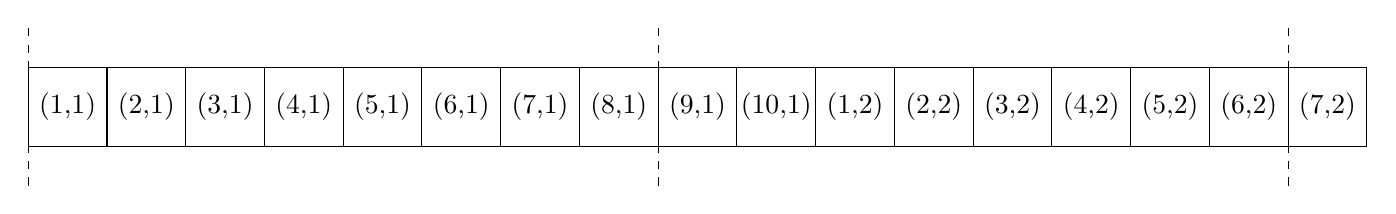
\begin{tikzpicture}
  \draw[step=1cm] (0,0) grid (17,1);
  \foreach \i in {0,8,16} {
    \draw[dashed] (\i,-.5) -- (\i,1.5);
  }
  \foreach \i in {1,...,10} {
    \draw (\i-0.5, 0.5) node {(\i,1)};
  }
  \foreach \i in {1,...,7} {
    \draw (10+\i-0.5, 0.5) node {(\i,2)};
  }
\end{tikzpicture}
\end{adjustbox}

\begin{minted}[frame=single]{fortran}
do j = 1, 10
  !$omp simd aligned(A:64)
  do i = 1, 10
    A(i,j) = A(i,j) + ...
  end do
  !$omp end simd
end do
\end{minted}

\end{frame}
%-------------------------------------------------------------------------------

\begin{frame}
\frametitle{Aligning 2D arrays}

\begin{adjustbox}{max width={\textwidth}}
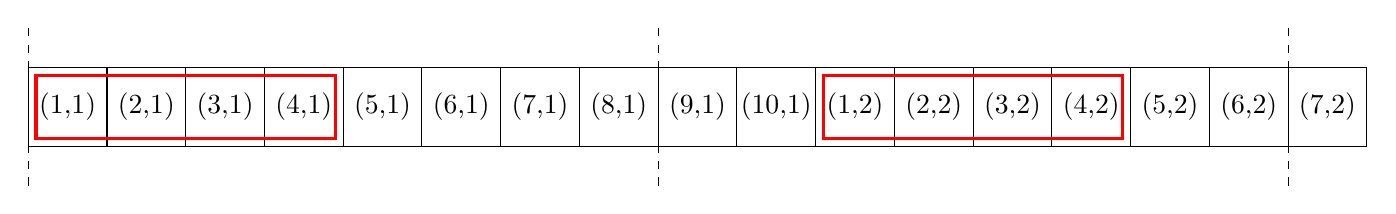
\begin{tikzpicture}
  \draw[step=1cm] (0,0) grid (17,1);
  \foreach \i in {0,8,16} {
    \draw[dashed] (\i,-.5) -- (\i,1.5);
  }
  \foreach \i in {1,...,10} {
    \draw (\i-0.5, 0.5) node {(\i,1)};
  }
  \foreach \i in {1,...,7} {
    \draw (10+\i-0.5, 0.5) node {(\i,2)};
  }

  \draw<2>[red, very thick] (0.1,0.1) rectangle (3.9, 0.9);
  \draw<3>[red, very thick] (10.1,0.1) rectangle (13.9, 0.9);
\end{tikzpicture}
\end{adjustbox}

\begin{itemize}
  \item The array is aligned to a 64-byte cache line.
  \item<2-> Accessing the vector \mintinline{fortran}|A(1:4,1)| is aligned.
  \item<3-> Accessing the vector \mintinline{fortran}|A(1:4,2)| is \emph{not} aligned.
  \vfill
  \item<4-> Need the inner stride to be a multiple of the alignment, and need to tell the compiler this is true (previous slide).
  \item<4-> Solution: pad the array, but beware of memory footprint.
  \item<4-> Example of why the \mintinline{fortran}|aligned| clause doesn't always ensure aligned load/stores.
\end{itemize}

\end{frame}
%-------------------------------------------------------------------------------

\section{Branches}
\begin{frame}
\frametitle{Branches}
\begin{itemize}
  \item CPUs support speculative execution, GPUs tend not to.
  \item Branch instructions have high latency.
  \item GPUs hide this latency by fast context switching, CPUs by good branch predictors.
  \item In both cases, divergent execution within the vector unit reduces performance.
  \item Can use predication, selection and masking to convert conditional control flow into straight line code.
\end{itemize}
\end{frame}

%-------------------------------------------------------------------------------
\begin{frame}[fragile]
\frametitle{Removing branches}
\begin{columns}

\begin{column}{0.5\textwidth}
Conditional execution
\begin{itemize}
  \item Only evaluate expression if condition is met
\end{itemize}
\begin{minted}[frame=single]{fortran}
if (a .gt. b) then
  acc = acc + (a - b*c)
end if
\end{minted}

\begin{minted}[frame=single]{C}
if (a > b)
  acc += a - b*c;
\end{minted}
\end{column}

\begin{column}{0.5\textwidth}
Selection and masking
\begin{itemize}
  \item Always evaluate expression and mask result
\end{itemize}
\begin{minted}[frame=single,breaklines]{fortran}
temp = a - b*c
mask = merge(1.0, 0.0, a .gt. b)
acc = acc + (mask * temp)
\end{minted}

\begin{minted}[frame=single]{C}
temp = a - b*c;
mask = a > b ? 1.0 : 0.0;
acc += mask * temp;
\end{minted}
\end{column}

\end{columns}
In practice, you may or may not see an improvement: the compiler may be doing something smart already.
\end{frame}

%-------------------------------------------------------------------------------
\section{Exercise}
\begin{frame}
\frametitle{Exercise}
\begin{itemize}
  \item Take your parallel 5-point stencil code and optimise.
  \item Think about:
    \begin{itemize}
      \item Memory access patterns
      \item Vectorisation
    \end{itemize}
  \item Note down the performance differences your optimisations make.
  \item Extension: consider these optimisaions for the Jacobi solver.
\end{itemize}
\end{frame}

%-------------------------------------------------------------------------------
\section{Summary}
\begin{frame}
\frametitle{Summary}

\begin{itemize}
  \item Performance of cache hierarchy.
  \item Performance analysis with the Roofline model.
  \item Vectorisation:
    \begin{itemize}
      \item Compiler auto-vectorisation.
      \item OpenMP \mintinline{fortran}|simd| construct.
      \item Memory access patterns.
      \item Data alignment.
    \end{itemize}

  \vfill

  \item Next sessions:
    \begin{enumerate}
      \setcounter{enumi}{3}
      \item NUMA and MPI interoperability.
      \item GPU programming with OpenMP.
      \item Tasks and Tools.
    \end{enumerate}
\end{itemize}


\end{frame}

%-------------------------------------------------------------------------------

\end{document}
